\section{Problem Definition}

In this section, we will define our ride sharing models. Given a trip request, and a set of taxi drivers, our goal is to assign the trip request to a driver satisfying the dynamic constraints while at the same time calculating the travel fare. 
%Next we define rider request, driver, price models (user and rider profiles), and our optimization goals.

\subsection{Basic Concepts}
The road network is represented as a graph $G(V, E)$, where each node represents intersections, and each edge represents a road segment. 
Each edge $(u,v) \in E$ $(u, v \in V)$ is associated with a weight $c(u,v)$ which is a travel cost (can be time or distance) from $u$ to $v$.
% TODO: define path in road network
The shortest path cost $d(s,t)$ is defined as minimal cost paths connect $s$ and $t$. In this paper, time and distance can be converted from one to the other.

\begin{definition}
(Ride request r) A ride request $<s, e, w, f>$ consists of a starting point $s \in V$ and an end point $e \in V$. Each request also specifies a maximal waiting time $w$, defining the maximal time the rider can wait after making a request, and a rider profile $f$, defining the expected discount ratio of ride sharing based on the extra detour.
%the ridesharing fare she would accept based on the extra detour and the shortest possible trip.
\end{definition}

When one ride request is accepted, it is assigned to a driver. One driver is driving a vehicle on road network with the accepted ride requests $TR<r_1, r_2, \cdots, r_n>$. A driver is also associated with a driver profile which defines the criteria of whether to accept a new request based on the expected total profit.

Given a set of ride requests $TR$ for a driver, a schedule of these ride requests $S=<x_1, \cdots, x_{2n}>$ is an ordered sequence of pickup and delivery points, where the origin of one ride must precede its destination. The driver will follow the sequence of picking up and dropping off riders. The schedule is changing over time. A schedule is valid if it satisfies the following conditions:

\begin{definition}
(valid schedule) A valid schedule $S$ satisfies the following constraints:
\begin{itemize}
	\item waiting time constraint.
	\item capacity constraint.
	\item profit constraint, which is the price constraint based on rider and driver profiles.
\end{itemize}
\end{definition}

Given a real-time ride $r$, and a set of cars on the road network, the objective is to match the ride to a car with particular optimization goal. Different optimization goals such as detour cost have been studied. In this paper, our aim is to design a sustainable price model and maximize the total profit. 

\subsection{Profit Model}
In general, the charge of one rider $r$ is based on the shortest distance $d$ between $r.s$ to $r.e$, i.e., fare(r) = F(d). Intuitively, with ridesharing, the charge of one passenger should be less than the normal fare if extra detour is incurred. Here the detour $\Delta d=d'(r.s, r.e)-d(r.s, r.e)$, where $d'$ is the actual distance between origin and destination. Consequently a discount would occur for a rider with respect to the extra detour: the more detour, the more discount of the fare.

\begin{definition}
	Rider profile is a function $f$ of extra detour $\Delta d$, which decides the discount ratio of a ride sharing request.
\end{definition}
The rider profile function can have different formations: linear decay, exponential decay etc. For example, $f(\Delta d)=c e^{-\lambda \Delta d}$.
Figure~\ref{fig:rider_profile} shows an example of rider profile.

\begin{figure}[!ht]
	\centering
	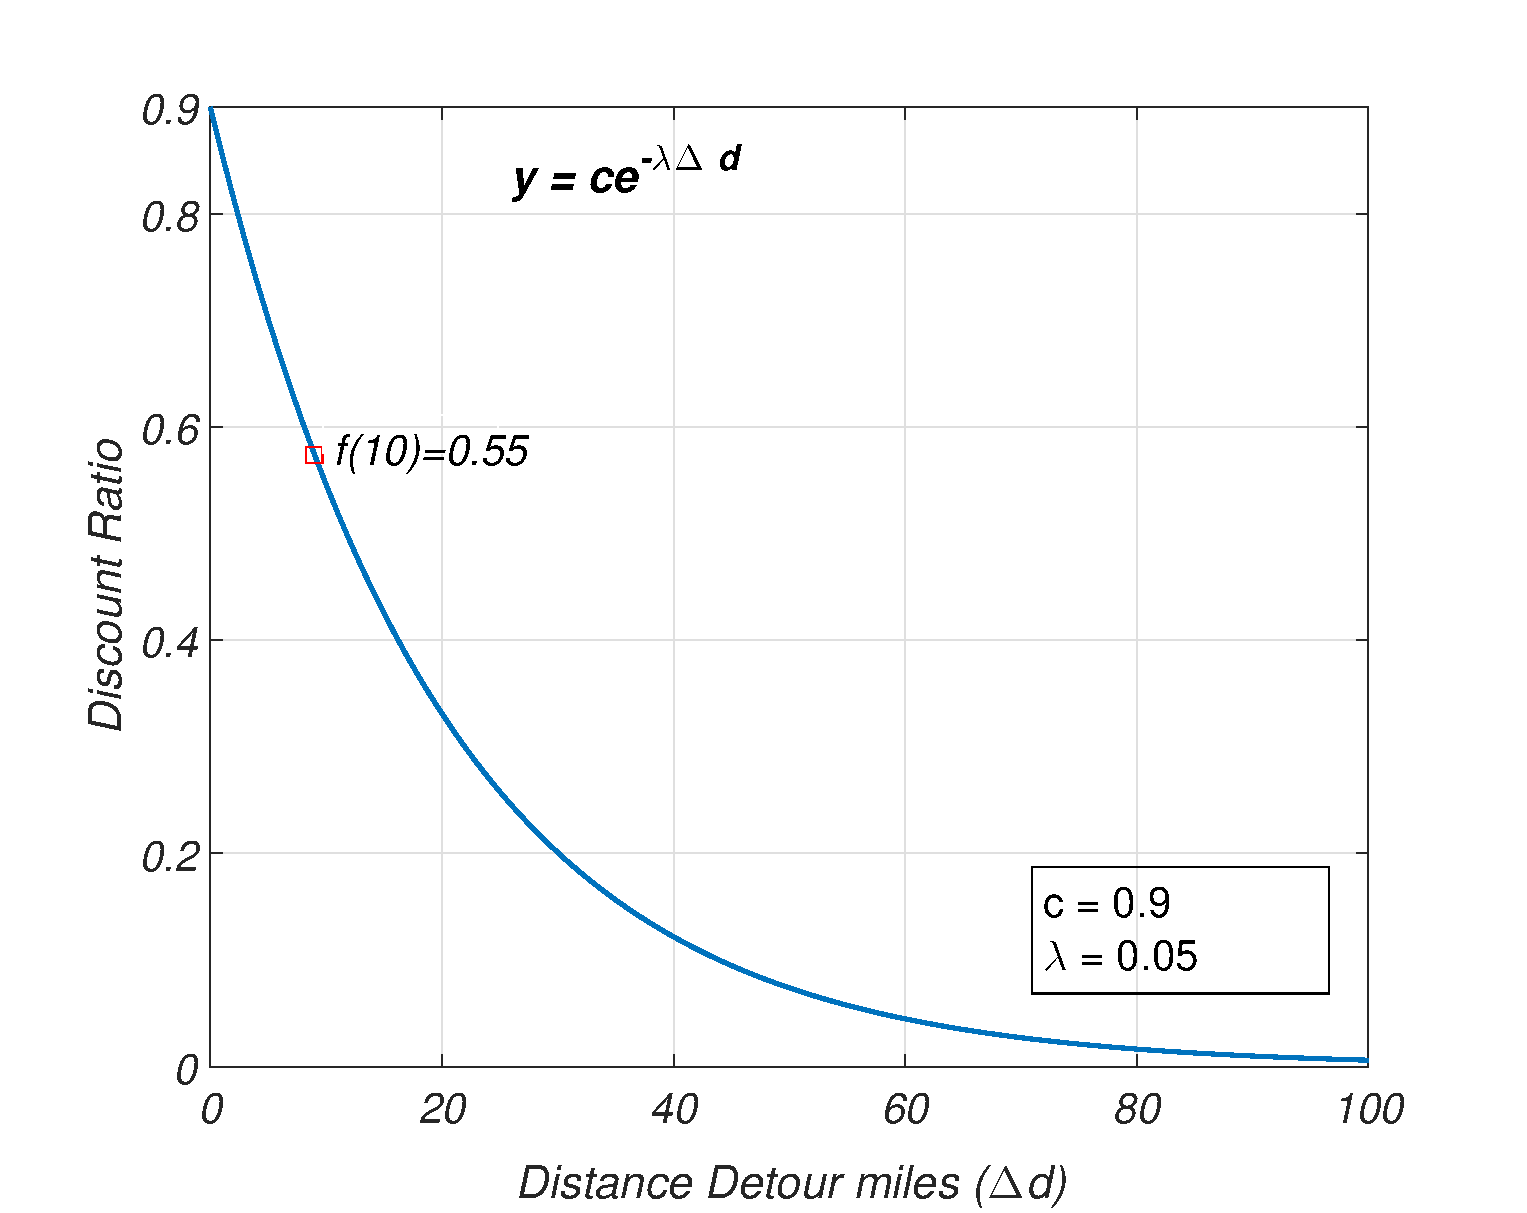
\includegraphics[width = 60mm]{fig/rider.eps}
	\vspace{-0mm}\caption{Rider profile} \vspace{-2mm} \label{fig:rider_profile}
\end{figure}\vspace{-0mm}

With the rider profile, for a rider with original distance $d$ and extra travel distance $\Delta d$, the fare of this rider $fare(r) = F(d) f(\Delta d)$.

\begin{definition}
	Driver profile is a function $g$ of the total travel distance $D$, which defines the criteria of whether to accept a new request into the current schedule $S$.
\end{definition}


The driver can decide whether to accept this new rider based on the comparison between the expected profit $g(D)$ and the new profit of inserting new ride. g is a monotonic increasing function of the total travel distance. Figure~\ref{fig:driver_profile} shows an example of driver profile, which is a linear function of the total travel distance.

\begin{figure}[!ht]
	\centering
	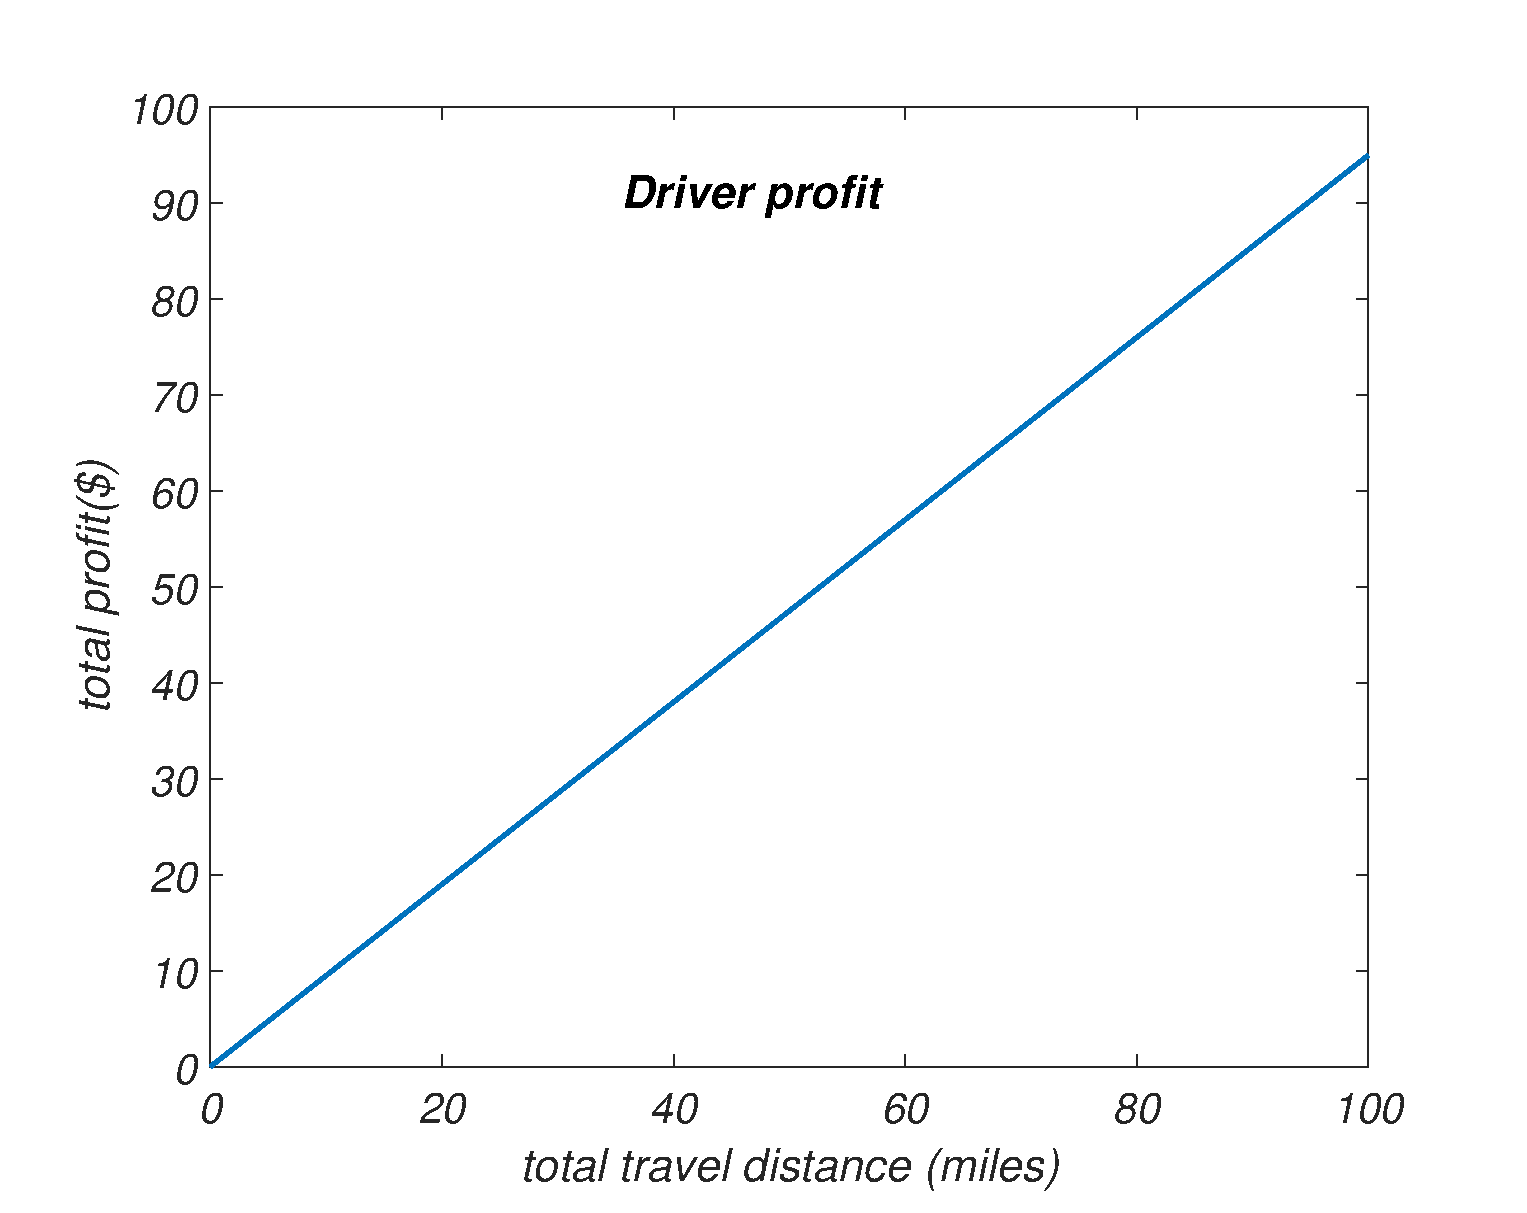
\includegraphics[width = 60mm]{fig/driver.eps}
	\vspace{-0mm}\caption{Driver profile} \vspace{-2mm} \label{fig:driver_profile}
\end{figure}\vspace{-0mm}
 

Suppose the original schedule of one car is $S(r_1, r_2, \cdots, r_n)$, and the total profit of driver is $M=\sum_{1}^{n}fare(r_i)$. After inserting new ride $r_{n+1}$, the total profit becomes $M'=\sum_{1}^{n+1}fare(r_i)$, and the total travel distance becomes $D$. If $M' \geq g(D)$, the driver accepts this new request, otherwise the driver rejects this new request. Hence, the extra profit of including the new rider becomes $M'-M$.

\begin{definition}
Define a Q function to calculate the profit from the driver's total profit.
\end{definition}

\subsection{Objective Function And Problem Definition}
Given a set of vehicles on the road network $G$ and a new incoming ride $r$, the problem is to find the vehicle which maximizes the extra profit of accepting the ride.

\textbf{Justify that our objective function is different with minimizing the travel cost.}

%%% TODO: given a rider and the current schedule, calculate the extra profit of inserting a new request.


%Properties of the above definition, can we guarantee the extra profit should be positive?

